\tikzstyle{document} = [circle, rounded corners ,text centered, draw=black]
\tikzstyle{corpus} = [draw,thick,minimum width=1cm,minimum height=4cm]
\tikzstyle{tf-idf} = [draw,thick,minimum width=1cm,minimum height=1cm]

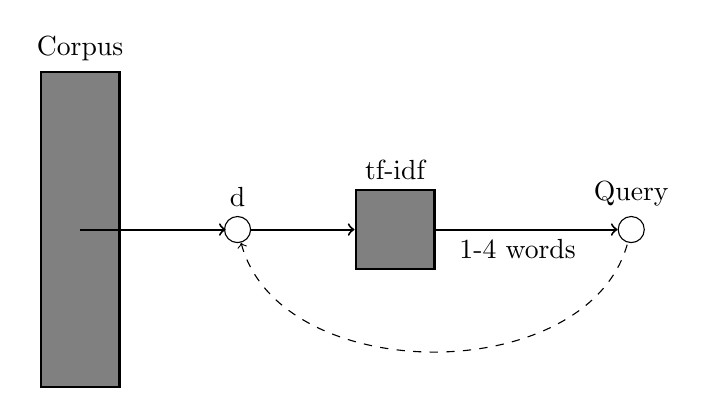
\begin{tikzpicture}
    \node [fill=gray, label={Corpus}] (corpus) at (0,0) [corpus] {};
    \onslide<2->{
        \node [document, label={d}] (doc) at (2, 0) {};
        \draw [line width=0.25mm, ->] (0,0) -> (1.85,0) node [right] {};
    };
    \onslide<3->{
        \node [fill=gray, label={tf-idf}] (tf-idf) at (4,0) [tf-idf] {};
        \draw [line width=0.25mm, ->] (doc) -> (tf-idf)  {};
    };
    \onslide<4->{
        \node [document, label={Query}] (Query) at  (7, 0) {};
        \draw [line width=0.25mm, ->] (tf-idf) -- node[below] {$1$-$4$ words} ++(2.6,0) -- (Query);
    };
    \onslide<5->{
        \path (doc) edge[bend right=75, dashed, <-] node [left] {} (Query);
    }
\end{tikzpicture}